%%% The main file. It contains definitions of basic parameters and includes all other parts.

% Meta-data of your thesis (please edit)
\input metadata.tex

% Generate metadata in XMP format for use by the pdfx package
\input xmp.tex

%% Settings for single-side (simplex) printing
% Margins: left 40mm, right 25mm, top and bottom 25mm
% (but beware, LaTeX adds 1in implicitly)
\documentclass[12pt,a4paper]{report}
\setlength\textwidth{145mm}
\setlength\textheight{247mm}
\setlength\oddsidemargin{15mm}
\setlength\evensidemargin{15mm}
\setlength\topmargin{0mm}
\setlength\headsep{0mm}
\setlength\headheight{0mm}
% \openright makes the following text appear on a right-hand page
\let\openright=\clearpage

%% Settings for two-sided (duplex) printing
% \documentclass[12pt,a4paper,twoside,openright]{report}
% \setlength\textwidth{145mm}
% \setlength\textheight{247mm}
% \setlength\oddsidemargin{14.2mm}
% \setlength\evensidemargin{0mm}
% \setlength\topmargin{0mm}
% \setlength\headsep{0mm}
% \setlength\headheight{0mm}
% \let\openright=\cleardoublepage

%% If the thesis has no printed version, symmetric margins look better
% \documentclass[12pt,a4paper]{report}
% \setlength\textwidth{145mm}
% \setlength\textheight{247mm}
% \setlength\oddsidemargin{10mm}
% \setlength\evensidemargin{10mm}
% \setlength\topmargin{0mm}
% \setlength\headsep{0mm}
% \setlength\headheight{0mm}
% \let\openright=\clearpage

%% Generate PDF/A-2u
\usepackage[a-2u]{pdfx}

%% Prefer Latin Modern fonts
\usepackage{lmodern}
% If we are not using LuaTeX, we need to set up character encoding:
\usepackage{iftex}
\ifpdftex
\usepackage[utf8]{inputenc}
\usepackage[T1]{fontenc}
\usepackage{textcomp}
\fi

%% Further useful packages (included in most LaTeX distributions)
\usepackage{amsmath}        % extensions for typesetting of math
\usepackage{amsfonts}       % math fonts
\usepackage{amsthm}         % theorems, definitions, etc.
\usepackage{bm}             % boldface symbols (\bm)
\usepackage{booktabs}       % improved horizontal lines in tables
\usepackage{caption}        % custom captions of floating objects
\usepackage{dcolumn}        % improved alignment of table columns
\usepackage{floatrow}       % custom float environments
\usepackage{graphicx}       % embedding of pictures
\usepackage{indentfirst}    % indent the first paragraph of a chapter
\usepackage[nopatch=item]{microtype}   % micro-typographic refinement
\usepackage{paralist}       % improved enumerate and itemize
\usepackage[nottoc]{tocbibind} % makes sure that bibliography and the lists
			    % of figures/tables are included in the table
			    % of contents
\usepackage{xcolor}         % typesetting in color

% The hyperref package for clickable links in PDF and also for storing
% metadata to PDF (including the table of contents).
% Most settings are pre-set by the pdfx package.
\hypersetup{unicode}
\hypersetup{breaklinks=true}

% Packages for computer science theses
\usepackage{algpseudocode}  % part of algorithmicx package
\usepackage{algorithm}
\usepackage{fancyvrb}       % improved verbatim environment
\usepackage{listings}       % pretty-printer of source code

% You might want to use cleveref for references
%\usepackage{cleveref}

% Set up formatting of bibliography (references to literature)
% Details can be adjusted in macros.tex.
%
% BEWARE: Different fields of research and different university departments
% have their own customs regarding bibliography. Consult the bibliography
% format with your supervisor.
%
% The basic format according to the ISO 690 standard with numbered references
\usepackage[natbib,style=iso-numeric,sorting=none,backend=bibtex]{biblatex}
% ISO 690 with alphanumeric references (abbreviations of authors' names)
%\usepackage[natbib,style=iso-alphabetic]{biblatex}
% ISO 690 with references Author (year)
%\usepackage[natbib,style=iso-authoryear]{biblatex}
%
% Some fields of research prefer a simple format with numbered references
% (sorting=none tells that bibliography should be listed in citation order)
%\usepackage[natbib,style=numeric,sorting=none]{biblatex}
% Numbered references, but [1,2,3,4,5] is compressed to [1-5]
%\usepackage[natbib,style=numeric-comp,sorting=none]{biblatex}
% A simple format with alphanumeric references:
%\usepackage[natbib,style=alphabetic]{biblatex}

% Load the file with bibliography entries
\addbibresource{bibliography.bib}

% Our definitions of macros (see description inside)
\input macros.tex

%%% Title page and various mandatory informational pages
\begin{document}
%%% Title page of the thesis and other mandatory pages

%%% Inscriptions at the opening page of the hard cover

% We usually do not typeset the hard cover, but if you want to do it, change \iffalse to \iftrue
\iffalse

\pagestyle{empty}
\hypersetup{pageanchor=false}
\begin{center}

\large
Charles University

\medskip

Faculty of Mathematics and Physics

\vfill

{\huge\bf\ThesisTypeTitle}

\vfill

{\huge\bf\ThesisTitle\par}

\vfill
\vfill

\hbox to \hsize{\YearSubmitted\hfil \ThesisAuthor}

\end{center}

\newpage\openright
\setcounter{page}{1}

\fi

%%% Title page of the thesis

\pagestyle{empty}
\hypersetup{pageanchor=false}
\begin{center}

\centerline{\mbox{
\includegraphics[width=166mm]{img/logo-en.pdf}}}

\vspace{-8mm}
\vfill

{\bf\Large\ThesisTypeTitle}

\vfill

{\LARGE\ThesisAuthor}

\vspace{15mm}

{\LARGE\bfseries\ThesisTitle\par}

\vfill

\Department

\vfill

{
\centerline{\vbox{\halign{\hbox to 0.45\hsize{\hfil #}&\hskip 0.5em\parbox[t]{0.45\hsize}{\raggedright #}\cr
Supervisor of the \ThesisTypeName{} thesis:&\Supervisor \cr
\ifx\ThesisType\TypeRig\else
\noalign{\vspace{2mm}}
Study programme:&\StudyProgramme \cr
\fi
}}}}

\vfill

Prague \YearSubmitted

\end{center}

\newpage

%%% A page with a solemn declaration to the thesis

\openright
\hypersetup{pageanchor=true}
\vglue 0pt plus 1fill

\noindent
I declare that I carried out this \ThesisTypeName{} thesis on my own, and only with the cited
sources, literature and other professional sources.
I understand that my work relates to the rights and obligations under the Act No.~121/2000 Sb.,
the Copyright Act, as amended, in particular the fact that the Charles
University has the right to conclude a license agreement on the use of this
work as a school work pursuant to Section 60 subsection 1 of the Copyright~Act.

\vspace{10mm}

\hbox{\hbox to 0.5\hsize{%
In \hbox to 6em{\dotfill} date \hbox to 6em{\dotfill}
\hss}\hbox to 0.5\hsize{\dotfill\quad}}
\smallskip
\hbox{\hbox to 0.5\hsize{}\hbox to 0.5\hsize{\hfil Author's signature\hfil}}

\vspace{20mm}
\newpage

%%% Dedication

\openright

\noindent
\Dedication

\newpage

%%% Mandatory information page of the thesis

\openright
{\InfoPageFont

\vtop to 0.5\vsize{
\setlength\parindent{0mm}
\setlength\parskip{5mm}

Title:
\ThesisTitle

Author:
\ThesisAuthor

\DeptType:
\Department

Supervisor:
\Supervisor, \SupervisorsDepartment

Abstract:
\Abstract

Keywords:
{\def\sep{\unskip, }\ThesisKeywords}

\vfil
}

% In Czech study programmes, it is mandatory to include Czech meta-data:

\ifx\StudyLanguage\LangCS

\vtop to 0.49\vsize{
\setlength\parindent{0mm}
\setlength\parskip{5mm}

Název práce:
\ThesisTitleCS

Autor:
\ThesisAuthor

\DeptTypeCS:
\DepartmentCS

Vedoucí diplomové práce:
\Supervisor, \SupervisorsDepartmentCS

Abstrakt:
\AbstractCS

Klíčová slova:
{\def\sep{\unskip, }\ThesisKeywordsCS}

\vfil
}

\fi

}

\newpage

%%% Further pages will be numbered
\pagestyle{plain}


%%% A page with automatically generated table of contents of the thesis

\tableofcontents

%%% Each chapter is kept in a separate file
\chapter*{Introduction}
\addcontentsline{toc}{chapter}{Introduction}


\section*{Motivation}

Domain modeling is fundamental both in data and software engineering. Domain modeling techniques, such as conceptual modeling techniques, where a domain model is expressed as an ER or UML class diagram, or ontology engineering techniques, which define a domain model as a domain ontology, are well established both in academia and industry \cite{Verdonck2018}. However, creating these domain models manually takes a non-trivial amount of time and requires trained experts. Therefore, various modeling automation techniques have been proposed \cite{Sonbol2022}. Recently, researchers began to evaluate different approaches to using large language models (LLMs) as possible automation solutions \cite{Chen2023,Saeedizade2024}.


\section*{Solution approach discussion}

Currently, fully automated domain modeling with LLMs works only for simple domain descriptions with a small number of domain elements \cite{Camara2023}. This is true even when advanced prompting techniques are applied \cite{Chen2023,Saeedizade2024}. To mitigate this issue, the user can be introduced into the domain modeling process \cite{Camara2023} and the LLM can be used as an assistant. For example, \citet{Camara2023} experimented with domain modeling in a conversation dialogue fashion with the ChatGPT-3.5. First, the LLM generated some preliminary domain model and then the authors created follow-up instructions to edit their domain models. However, as the LLM executed directly each authors' instruction, this frequently led to back-and-forth communication as the authors tried correcting the mistakes made by the LLM in the previous steps. Additionally, there was no option to manually model any parts of the domain model to help the LLM model the parts it struggled with. For a detailed description of related work see chapter \ref{chap:related_work}.


\section*{Using LLM as an assistant}
\label{section:llm_as_an_assistant}

Recently, a lot of applications started using the LLM as an assistant. Here is a list of some of those applications with a brief description of the assistant usage.

\begin{itemize}
\item \textit{Grammarly}\footnote{\url{https://app.grammarly.com/}}: assistant for writing
\item \textit{GitHub Copilot}\footnote{\url{https://github.com/features/copilot}}: assistant for programming
\item \textit{Notion AI}\footnote{\url{https://www.notion.so/help/guides/category/ai}}: assistant for taking notes
\end{itemize}

These applications have the following features in common. First, the LLM usually provides only suggestions to the users. These suggestions usually can be accepted or rejected or in some cases, a new suggestion can be re-generated. The reason for this behaviour is that the LLMs still make a lot of mistakes so direct application of their output is usually not wanted. Typically, these applications explicitly warn their users that the generated output can provide false, biased and outdated information. Furthermore, if these mistakes are not removed by the users these mistakes can accumulate over time and can lead to even worse output performance. Second, the suggestions are usually in a form such that the users can quickly decide if they want to use them. For example, in \textit{Grammarly} the spell-checking feature represents each suggestion as an underlined text that contains a reason why it was underlined and a suggested correction. In \textit{GitHub Copilot} especially in the hands of an experienced developer, it is usually easy to decide if a suggested piece of code or a suggested code documentation is appropriate based on the surrounding context. And finally, in \textit{Notion AI} suggested notes are usually easy to evaluate as they are typically clearly structured.


\section*{Areas with lack of research}

Based on our exploration, the following areas have a lack of research and can have a significant impact on making the domain modeling process faster and more accessible:

\begin{itemize}
\item manual domain modeling extended with the LLM as an assistant that only provides suggestions
\item using techniques for filtering domain descriptions such as retrieval-augmented generation to improve the performance of LLMs for the domain modeling tasks
\item using real-life domain descriptions for evaluating domain modeling tasks with LLMs
\item creating a tool for demonstrating the viability of the selected approach
\end{itemize}


\section*{Goals}

The domain modeling process typically follows a systematic approach. First, the domain experts create an unstructured domain description, and second, the modeling experts solely based on this domain description create an exact, structured, and formalized domain model.

This thesis aims to help with the second step and address the mentioned areas with lack of research by creating a tool for domain modeling where the LLM assistant cooperates with a human modeling expert. The modeling expert provides an unstructured domain description as input into the domain modeling process and the assistant generates suggestions solely based on this domain description.

To improve the performance of the LLM, we divide the domain modeling process into a set of simpler steps and we employ the retrieval-augmented generation technique for providing only the relevant parts of the domain description based on the given task to the LLM. This assistant always generates output in the form of suggestions as the LLMs still frequently make mistakes. To help the users decide if they want to apply the generated suggestions, we highlight each suggested domain element in the given domain description. Finally, we experimentally evaluate our approach with a real-life domain descriptions.

This LLM assistant is mainly intended to help the users create their domain models faster and to help them better document their domain models. This assistant should be:

\begin{enumerate}
\item intuitive to use
\item suggesting mostly appropriate classes, attributes, and associations
\item suggesting mostly appropriate descriptions of classes, attributes, and associations
\item able to summarize a selected part of a domain model
\item able to highlight in the given domain description the parts that the user already modeled
\item able to generate corresponding suggestions in a few seconds
\end{enumerate}


\section*{Outline}

Chapter \ref{chap:background} provides an overview of the basic technologies that we will be using.
Chapter \ref{chap:domain_modeling_process_analysis} introduces the minimalist but necessary formalization of the domain modeling process and its steps that can be automated.
Chapter \ref{chap:framework} describes a theoretical generic framework for building LLM-based domain modeling assistants.
Chapter \ref{chap:framework_configuration} shows some possible configurations of the framework.
Chapter \ref{chap:protype_software_application} implements the framework with the proposed configurations.
Chapter \ref{chap:evaluation} presents the experimental evaluation of our framework implementation.
Chapter \ref{chap:development_documentation} contains the development documentation and chapter \ref{chap:user_documentation} contains the user documentation. Chapter \ref{chap:related_work} gives an overview of the related work and chapter \ref{chap:conclusion} concludes our work and suggests possible future work.
\chapter{Domain modeling process analysis}
\label{chap:domain_modeling_process_analysis}

In our thesis, we consider a domain modeling process starting with a domain description $T$ acquired from stakeholders and knowledge sources such as internal documentation, manuals, or state law. $T$ can be a well-curated text, but it may also encompass varied interpretations articulated by different stakeholders at various levels of detail. A modeling expert translates $T$ into a domain model $M$ in a sequence of steps.

A domain model $M = (\mathcal{C}, \mathcal{P})$ consists of a set of classes $\mathcal{C}$ and properties $\mathcal{P}$.

A class $C \in \mathcal{C}$ has its $name(C)$ that identifies $C$ in $M$ and briefly characterizes the semantics of $C$. The class $C$ also has a $description(C)$ that describes the semantics of $C$.

A property $P \in \mathcal{P}$ has also $name(P)$ and $description(P)$ used for the same purposes. It has a $cardinality(P)$ that refers to the specification of the number of instances of one domain element that can or must be associated with each instance of some class. It also has a source class, such that $source(P) \in \mathcal{C}$ and it can have a target class such that $target(P) \in \mathcal{C}$. $P$ is a binary association if $target(P)$ is defined otherwise, $P$ is an attribute. If $P$ is an attribute, then it also has $dataType(P)$ which defines the data type of $P$.

These basic modeling constructs are prevalent in real conceptual models \cite{Keet2015}, so their automation could have a significant impact. We distinguish the following steps.


\section{Steps}
\label{sec:modeling_steps}

\begin{description}
\item [Design a class] For a concept in $T$, create a class $C$ with a designated $name(C)$.

\item[Design an attribute for a class] For a class $C$ and a concept in $T$ that characterizes $C$, create an attribute $P$, where $C = source(P)$, and define its $name(P)$.

\item[Design an association for a class] For a class $C$ and a concept in $T$ that describes a relationship of $C$ with another concept, create an association $P$ such that $C = source(P)$ or $C = target(P)$, and define its $name(P)$. If not yet represented, create a class $D$ for the other concept and specify its $name(D)$.

\item [Design a description for a class] For a class $C$ and a concept in $T$ that characterizes $C$, define $description(C)$.

\item [Design a description for an attribute] For an attribute $P$ and a concept in $T$ that characterizes $P$, define $description(P)$.

\item [Design a description for an association] For an association $P$ and a concept in $T$ that characterizes $P$, define $description(P)$.

\item [Design a data type for an attribute] For an attribute $P$ and a concept in $T$ that characterizes $P$, define $dataType(P)$.

\item [Design a cardinality for an attribute] For an attribute $P$ and a concept in $T$ that characterizes $P$, define $cardinality(P)$.

\item [Design a cardinality for an association] For an association $P$ and a concept in $T$ that characterizes $P$, define $cardinality(P)$.
\end{description}


\section{Example}
\label{sec:simple_domain_description_example}

Consider the following domain description: ``\textit{In this company, every employee works in some department. Each employee is uniquely identified by his ID.}'' Figure \ref{fig:simple-employee-domain-model} shows how a corresponding domain model can look like. It contains the class \textit{employee} with the attribute \textit{ID} and the association \textit{works in} between the classes \textit{employee} and \textit{department}.

\begin{figure}[!h]
    \centering
    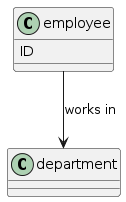
\includegraphics[scale=0.65]{img/domain-modeling-steps-example.png}
    \caption{\centering Simple domain model example}
    \label{fig:simple-employee-domain-model}
\end{figure}

To create the described domain model when starting from an empty domain model, the following steps can be executed:

\begin{enumerate}
\item design a class: for the concept ``\textit{In this company, every employee works in some department}'' create the class $C$ such that \textit{employee} = $name(C)$
\item design a class: for the concept ``\textit{every employee works in some department}'' create the class $C$ such that \textit{department} = $name(C)$
\item design an attribute: for the class \textit{employee} and the concept ``\textit{Each employee is uniquely identified by his ID}'' create the attribute $P$ such that \textit{ID} = $name(P)$ and \textit{employee} = $source(P)$
\item design an association: for a class \textit{employee} and the concept ``\textit{every employee works in some department}'' create the association $P$ such that \textit{works in} = $name(P)$, \textit{employee} = $source(P)$ and \textit{department} = $target(P)$
\end{enumerate}

For providing more information for this domain model, the other mentioned steps can be used to define descriptions of the modeled elements, to define data types of the modeled attributes, and to define cardinalities of the modeled attributes and associations.
\chapter{Related work}
\label{chap:related_work}

The difficulty of domain modeling has long been a well-known problem that has been the focus of many authors \cite{Bossung2007}.
We can observe two research directions, one exploring the methodological possibilities of allowing domain experts to create domain models without requiring modeling expertise \cite{Bossung2007,Denaux2011,Ionita2015}, the other focusing on domain modeling automation \cite{Arora2016,Saeedizade2024,Lucassen2017,Burgueno2021}.

In previous research on domain modeling automation, we can identify rule-based and machine learning methods.
In the rule-based field, \citet{Arora2016} studied rule-based methods for the extraction of models from the specification of requirements in the natural language (NL) and provided a comprehensive overview of the existing rule-based methods up to date.
%They distinguished rules for concept extraction, associations and generalization extraction, cardinalities extraction, and attributes extraction.
%The rules were based on the linguistic syntactical analysis of the NL sentences, e.g. nouns in subject/object positions, verbs, genitives, and adjectives, etc.
The paper also introduced novel extraction rules that better exploit linguistic dependency information from NLP parsers with link paths, a series of syntactic dependencies in a sentence that connect two concepts indirectly through one or more intermediate concepts.
The focus on complex NLP rules was later criticized in \cite{Lucassen2017} where the authors proposed a simpler approach to extract domain models from user requirements expressed as user stories (requirements in the form of \emph{As a <who>, I want <what>, so that <why>.})
%Even less expressive than unrestricted domain descriptions, user stories are a popular way to express user requirements in practice.
Later works elaborated further on this approach, e.g. \citet{Nasiri2021}, with more recent \citet{Gupta2023} that considers so-called Behavior-Driven Development scenarios that extend user stories but they are still simpler than NL.
Recently, \citet{Burgueno2021} focused on assisting modeling experts by generating potential new model elements to be added to an existing one instead of generating full models.
Recent field surveys are available for further details by \citet{Raharjana2021} and \citet{Sonbol2022}.

\citet{Burgueno2021} complement the rule-based approach by identifying relevant parts of NL descriptions using word embeddings.
This leads us to another family of domain model extraction techniques that are based on machine learning (ML).
\citet{Saini2020,Saini2020a,Saini2020b} introduced a technique that extends the NLP rule-based techniques with ML classifiers such as Linear Discriminant Analysis and Logistic Regression to predict concept categories and types, and Bidirectional Long Short-Term Memory (BiLSTM) neural network model to determine relationships, cardinalities, and patterns among domain concepts in clusters of sentences describing semantic concepts in domain descriptions.
The authors then extended this approach with a bot-assisted approach that provides interactive support to domain modelers by generating multiple possible solutions for the given descriptions and incrementally adapting to the domain modeler's decisions \cite{Saini2022}.
\citet{Yang2022} describe another approach that combines NLP, rule-based concept extraction, and ML. It describes a classifier that labels sentences as describing a class or a relationship. Handwritten rules are then applied to parse English sentences to extract fragments of UML class diagrams, which are then merged.

Recent advances in the field of LLMs have directed the attention of researchers towards exploring the possibilities of using them to automate domain modeling. \citet{Fill2023} conducted early experiments using ChatGPT based on GPT-4 models \cite{Achiam2023} to show how to generate domain models. They show basic prompt templates and demonstrate on simple domain description examples that the model is able to generate ER and UML class diagrams in a structured JSON format.
They also experiment with process models.
\citet{Camara2023} also analyze the possible use of ChatGPT as a domain modeling assistant. The analysis is based on two experiments.
The first was based on individual interaction of the authors with ChatGPT who wrote prompts asking ChatGPT to create models of different size (10 to 40 classes+associations) based on short domain descriptions.
The second was based on comparing the domain models generated by ChatGPT with predesigned domain models. The authors showed that the performance of the ChatGPT (in Feb 2023 version) was not as good as it was observed in the field of programming code generation. The experiments demonstrated the ability of ChatGPT to correctly generate only models with fewer than 8-10 classes. However, they also demonstrated that the interaction with the ChatGPT to build the model incrementally improves the results.
%The authors also described the qualitative differences between different domains, probably caused by the fact that these domains were represented at different levels of detail in the training data.
\citet{Chen2023} provided the first systematic analysis of the capabilities of LLMs to generate domain models from textual descriptions using different prompting strategies. The authors focused on the task of generating a domain model from the given domain description without interaction with the user. They describe a versatile architecture that supports different prompt engineering techniques (CoT, N-shot prompting), different LLMs (GPT-3.5, GPT-4 in the paper, but the architecture is not limited to this), and different domain modeling constructs on the output.
The paper also presents an experimental evaluation of the proposed architecture. Using eight domain descriptions from the authors' university courses, corresponding manually created reference domain models (7-23 classes, 11-43 attributes, 9-27 associations) and LLM outputs manually compared to the reference models, they demonstrated the F1 scores 0.76 for classes, 0.61 for attributes, and 0.34 for relationships, concluding that LLMs are still impractical for fully automated modeling.

The field of domain modeling automation is related to the field of \emph{ontology learning} (OL)\cite{Konys2019,Khadir2021}, which includes not only the automated extraction of domain models from unstructured text, but also from other sources, such as structured data \cite{Lakzaei2021}.
\citet{Neuhaus2023} concludes that LLMs can be helpful to ontology engineers when designing their domain models as ontologies. However, we should not expect the output of an LLM to reflect a logically consistent and sound view of any given domain, because the training data of any LLM likely contain a variety of divergent views on any given subject matter.
Recently, \citet{BabaeiGiglou2023} explored the potential of LLMs for OL through three partial OL tasks -- suggesting conceptual types for a given term, identifying ISA hierarchies between two types, and identifying non-ISA associations between two types. The tasks do not consider the domain description, but extract the domain model directly from the trained parameters of the LLM.
\citet{Saeedizade2024} investigated the potential of LLMs to help ontology engineers by generating OWL ontologies from ontological requirements.
Their study explored the efficacy of LLMs in the ontology modeling, focusing on multiple LLMs and various prompting techniques.
The authors structured their prompts into the header section with the task description, the helper section explaining the basic ontological construct and syntax, the story section with the domain description and ontology competency questions (CQs) and the footer section with cautionary advice to avoid common pitfalls in ontology design.
The evaluation involved comparing the ontologies generated by the LLMs with student solutions based on their ability to address the given CQs.
The study concluded that only GPT-3.5 and GPT-4 produced reasonable OWL outputs.
In particular, GPT-4 outperformed the average quality of the student ontologies when the CQbyCQ prompting technique was used.
This technique splits individual CQs into separate prompts and merges their outputs into a single ontology.
However, the evaluation was performed on simple domain descriptions with short narratives in a single paragraph each with 15 competency questions.
%By adopting this approach, the study demonstrated that advanced LLMs, particularly GPT-4, hold significant promise to improve the efficiency and quality of ontology engineering. 
\chapter{LLM-based Modeling Assistant Framework}

We propose solving the automation of these domain modeling steps as text generation problems similarly to \citet{Chen2023}, where the authors consider a domain description $T$ with an underlying ground truth model $M$, and approach the problem of model generation as the problem of defining a text generator $f$ with $M' = f(T)$, where $M'$ is the generated model similar to $M$. The generator $f$ is an LLM-based operator defined by a predesigned prompt that instructs an LLM to return a structured textual representation of $M'$ for the input $T$. \\

TODO: Brief chapter description


\section{Generators}

We consider more fine-grained text generation problems solved by the following generators:

\textbf{Class generator}: $gen_c$ that for $T$ suggests classes $\{C_1, \ldots, C_n\}$ each with a suggested $name(Ci)$.

\textbf{Attribute generator}: $gen_a$ that for $T$ and a class $C$ suggests attributes $\{P_1, \ldots, P_n\}$, each with $source(P_i) = C$, suggested $name(P_i)$, and original text $orig(Pi)$ that is part of $T$ on which base $gen_a$ suggested $P_i$.

\textbf{Association generator 1}: $gen_r$ that for $T$ and a class $C$ suggests associations $\{P_1, \ldots, P_n\}$, each with $source(P_i) = C$ (or $target(Pi) = C$), suggested $name(Pi)$, and with the original text $orig(P_i)$ that is part of $T$ on which base $gen_r$ suggested $P_i$. It also suggests the other class $D$, with $target(Pi)= D$ (or $source(Pi) = D$), and suggested $name(D)$. \\

TODO: Association generator 2 \\

TODO: Description generator \\

TODO: Data type generator \\

TODO: Description generator \\


\chapter{Prompts}

TODO: Description of what we will discuss in this chapter.

\section{General rules}
As we use already existing LLMs we design our prompts in a way that resembles their training data as most as possible. Because usually most of the training data come from the internet we follow these rules:
\begin{itemize}
\item our prompts are only in English
\item unstructured data are in plain text format
\item structured data are in JSON format \
\end{itemize}

NOTE: Tady možná bych mohl napsat, že jako future work by se dal zkoumat vliv konkrétního strukturovaného formátu na kvalitu výstupu, tedy že dává smysl vyzkoušet i něco jiného než JSON \\~\\


\section{General tips}
There exists a lot of general tips for writing prompts independent on the chosen prompting technique. In our experience these tips helped mostly when working with less quality LLMs as the more quality LLMs are less sensitive to a slight differences in the prompt.

When developing our prompts we took inspiration mostly from the Microsoft's prompt engineering guide\footnote{\url{https://learn.microsoft.com/en-us/azure/ai-services/openai/concepts/advanced-prompt-engineering?pivots=programming-language-chat-completions}} and from OpenAI's prompt engineering guide\footnote{\url{https://platform.openai.com/docs/guides/prompt-engineering}}. In our experience the most notable tips are:



\subsection{Starting or ending with the most important instructions}
LLMs place the greatest emphasis on the information at the start and at the end of the prompt. Therefore, defining the main task at the start of the prompt and then repeating it at the end can increase the output quality.


\subsection{Adding clear consistent syntax}
Adding clear and consistent syntax makes the prompt more human readable and also can improve the output quality.


\subsection{Breaking the task down}
LLMs usually perform better when they are given order in which to generate the output. Also the order of the steps matter as the LLM generates the next token both based on the prompt and based on it's previous output.


%\subsubsection{Priming the output}
%In our experience the LLMs are usually trained in a way to start their response by some preliminary description of the output. This can be reduced by for example putting ``Output:'' at the end of the prompt.

TODO: Možná by se ty jednotlivé body hodilo jinak strukturovat, například mít jako název kapitoly prompts, aby potom ty subsekce byly 3.1.1, 3.1.2, atd.

TODO: Možná něco o tom, že LLM typicky kladou velký důraz na system message, proto je dobré sem také uvést hlavní instrukci \\

TODO: Projít si ty odkazy ve footnotech, jestli tam ještě nenajdu něco důležitého \\


\section{Structure}

As we saw the way the prompts are written greatly influences the quality of the LLM output thus our prompts are prepared in advance in form of a templates with placeholders that are later on replaced by the user's specific arguments. These templates have usually the following structure:

\begin{enumerate}
\item control instruction
\item modeling procedure
\item output specification
\item example specification
\item input specification \\
\end{enumerate}

TODO: každý item udělat jako referenci na příslušnou subsubsekci \\

TODO: asi zmínit, že tato struktura se týká hlavně generování tříd, atributů, asociací


\subsection{Control instruction}
The control instruction defines the main task. It is put at the start of the prompt so the LLM puts the most emphasis on this instruction and also from the same reason this instruction is sometimes repeated. If we want the LLM to respond solely based on the given input then the prompts starts with the words ``solely based on the given$\ldots$''

For example for generating attributes the control instruction can look like this:
``Solely based on the given context generate all attributes for the class: "\{source\_class\}".'' Where the ``\{source\_class\}'' is the mentioned placeholder that is replaced later on.

On the other hand, if want the LLM to extract the output only from it's trained parameters then for example the prompt for generating attributes can start with the words: ``Generate attributes for the class: "\{source\_class\}"''. \\

TODO: Tady možná by stačilo říct, že tam nedáváme to solely based on the given context \\


\subsection{Modeling procedure}
The modeling procedure provides step by step plan on how the LLM should generate the output. This the place suitable for experimenting with various prompt techniques such as chain of thoughts. \\

TODO: možná vysvětlit, že při generování návrhů, necháváme nejdřív vygenerovat original text (context) před vygenerování názvu návrhu. Ale toto možná dává smysl pouze pokud provedeme ruční měření kvality výstupů, protože nevím, jestli má smysl tady psát, že to tak dělá pouze, protože máme hypotézu, že je to lepší.


\subsection{Output specification}
Specifies output in JSON format so we can automatically parse the LLM output.


\subsection{Example specification}
Optionally, the prompt can contain examples of the input and corresponding output.


\subsection{Context specification}
Contains the input such as user's domain description or user's domain model. This is a place suitable for experimenting with various filtering algorithms for filtering the input to provide to the LLM only the necessary input that it needs for generating the wanted output to provide less opportunity for errors such as hallucination.


\section{Specific techniques}

There exists a lot of specific prompting techniques that can significantly improve the LLMs performance. Here we write about those that we experimented with.


\subsection{Chain of thoughts}

TODO: Zkusit najít nějakou definici, nebo aspoň vystihující popis. \\

TODO: Možná trochu více rozepsat, co je to CoT: "CoT prompting can be categorized into two major paradigms. One adds a single prompt like “Let’s think step by step”
 after the test question to facilitate the reasoning chains in LLMs" (zdroj: Automatic CoT prompting in LLMs) \\

TODO: Asi nejlepší bude uvést typický obrázek slovní úlohy, kde když LLM pouze generuje odpověď, tak dojde ke špatnému výsledku oproti variantě s cot. \\

TODO: potom můžu provést úvahu, jakým způsobem by se cot dalo aplikovat pro generování tříd, atribut, asociací \\

We came up with a simple CoT technique where the LLM is instructed to generate the  suggestion in JSON object step by step. This means that the LLM first generates single fields of this object and then it puts all those fields together into a one object. (TODO: Example) \\

This simple CoT technique improved output quality in terms of generating attributes and associations however, it decreased output quality when generating classes. \\

TODO: Možná vyjmenovat nějaké další možné přístupy, jako například automatic CoT, tu self-consistency CoT atd. \\


\subsection{Tree of thoughts}

TODO: Asi nějak navázat na to cot, ale že místo jedné myšlenky rozvíjíme více myšlenek najednou, což lze buď udělat v rámci jednoho promptu, nebo iterativně (ale to samé platí u CoT, takže možná to zmínit tam)


\subsection{N-shot prompting}

TODO: Nějaký basic popis. \\

Main advantages of this techniques are:

\begin{enumerate}
\item output quality improvement as LLM better understands the given task
\item more detailed specification of the output format
\item possible improvement of user experience for faster response time
\end{enumerate}

(1) output quality improvement as LLM better understands the given task. Especially when using lower quality LLM it can improve understanding of the given task by learning from the provided examples.

(2) more detailed specification of the output format provides for example the opportunity to define in what naming conventions the output fields should be. For example if the LLM generates class names without examples some of the names can be in snake case and some other in camel case. When providing examples with a consistent naming style the LLM then adopts this style. This also helps to for example define how the names should start with. For example without providing any example attribute names can sometimes start with ``has'' but with providing specific examples we can make the LLM to use only nouns for attribute names. \\

TODO: Zkusit lépe a jednodušeji strukturovat, možná je zbytečné rozepisovat dva příklady a zvládnu to dát do jednoho. \\

(3) in combination with some other prompting technique such as chain of thoughts the examples help us to specify in what order the final JSON objects should be outputted. For example with the specific examples we can instruct the LLM to output the JSON object one by one and not as a whole at the end so we can show the output faster to the user.

Further, it can be experimented with how many examples we insert into the prompt. Not enough examples can lead to LLM not understanding details of our task. However, too much examples can lead to over-training the LLM and leaking the inserted examples into the output or if we work with some smaller context window size the examples could fill in the available prompt length.
\chapter{Retrieval-augmented generation}
Initially, we introduce the concept of Retrieval-Augmented Generation (RAG). Following this, we elucidate the application of RAG within our specific framework. Subsequently, we delineate the challenges encountered during the implementation process and the strategies employed to address these issues.

\section{Motivation}
When a LLM generates output, it relies on its trained parameters, which may contain outdated information. This occurs because, after the training phase, these parameters are no longer updated. Consequently, the output produced by the LLM can be outdated or irrelevant. To address this issue, RAG can be employed to incorporate external knowledge into the LLM's output generation process.

\section{Basic RAG flow}
The RAG process typically involves three main steps: First, the creation of an external knowledge base. Second, the identification of relevant information within this knowledge base based on the user's input. And third, the generation of a prompt that combines the user's input with the retrieved relevant information from the external knowledge base. \cite{Gao2023} \\

NOTE: Jestli bude potřeba, tak ty jednotlivé body můžu klidně více rozepsat viz Indexing, Retrieval, Generation v \cite{Gao2023} \\

NOTE: Tady můžu nakreslit nějaký obrázek, obsahově by se sem hodilo něco jako \url{https://pvml.com/wp-content/uploads/2024/04/rag.png}


\section{How we use RAG}
In terms of our application the knowledge base is the user's domain description. When generating attributes and associations our goal is to find the relevant parts of this domain description based on the given source class and target class if it is provided.

For example, if in domain description the first sentence informs us about employees and the second sentence informs us about projects, when suggestion attributes for the class ``employee'' we insert only the first sentence in the prompt. This is mainly done to reduce the LLM's hallucination. But it can also help to reduce the prompt length when working with a domain description that does not fit into the LLM's context window size.



\section{Challenges}

Now we will describe the most significant challenges we encountered and the corresponding solutions we implemented to address them.

\subsection{Domain description segmentation}
First, we need to split the domain descriptions into chunks so for each chunk we can evaluate if it is relevant for the provided classes.

Determining the chunk size is a challenging task since with too big chunks we are risking having irrelevant parts of domain description in the prompt. On the other hand, with too small chunks we are risking that the chunks will be miss-classified as they will not contain enough information about their context for deciding if they are relevant.

In result, we consider each sentence of the domain description as a one chunk since it usually contains information about one thing and later on it is easy to concatenate the relevant chunks together simply by putting them next to each other in the original order from the domain description.


\subsection{Texts comparison}

Typically, as the first step in RAG the chunks are embedded into a vector database by usually some small-scale language model typically based on Bidirectional Encoder Representations from Transformers (BERT). And in the next step the user's instruction is embedded into the vector space with the same language model. Then the language model computes the distance between the embedded instruction and each of the chunks and the closest $k$ chunks are retrieved.

There are many language models that can be used for text embedding into a vector space. They mainly differ in their input format such as length of the input and whether the given query should be in form of a question or not. Also other methods can be used such as using the LLM to output the $k$ closest chunks. We use semantic and syntactic approach. We do not use some LLM for the text comparison as it usually takes many seconds to generate the output especially when in the worst case scenario the output can be very long when a large portion of the domain description has to be copied to the output.

The semantic approach uses the ``\textit{all-MiniLM-L6-v2}'' model\footnote{\url{https://huggingface.co/sentence-transformers/all-MiniLM-L6-v2}} that executes the described comparison in the vector space. It's intended use is a sentence and short paragraph encoder. As a comparison function we use cosine-similarity (TODO: Mám tady dát nějaký odkaz na cosine-similarity?).

The syntactic approach compares lemmas of the mentioned texts. We use the \textit{MorphoDiTa} tool \cite{Strakova2014} with the ``\textit{english-morphium-wsj-140407}'' model \cite{Straka2014}. As one word in a different contexts can have a different lemma, we lemmatize each word by word in isolation.


\subsection{Top k search}

In traditional RAG systems, a fixed number $k$ of the most relevant results are retrieved. However, in our specific application, $k$ is not a fixed number because the domain description may encompass a variable number of relevant sentences. To address this variability, we need to define the cosine-similarity threshold which is a value in between 0 and 1. The challenge lies in the fact that the computed cosine-similarity is always relative to the given input. Consequently, in one scenario, sentences with a cosine similarity higher than a certain threshold $x$ may be deemed relevant, while in another scenario, sentences with a cosine similarity higher than $x$ may be considered irrelevant.

We found out that our semantic RAG approach works a little bit better when setting the threshold based on the cosine-similarity of the most relevant sentence. This experiment can be found in the RAG evaluation section. (TODO: provide reference to the RAG evaluation section)


\subsection{Missing context}

Our segmentation into sentences can fail when for example some sentence contains pronoun referencing anything from a different sentence. For example consider this domain description: ``The book contains a lot of pages. It is very heavy.'' and input class named ``book''. Now when considering only the second sentence it doesn't contain any syntactic information about the book therefore it most probably would be discarded by any syntactic or semantic comparison algorithm even thought for example the attribute ``weight of the book'' could be derived from it.

One possible solution is to use some language model that can accurately solve the co-reference resolution task where each pronoun is replace with the corresponding words that are referenced. This way the previous example would look like this: ``The book contains a lot of pages. The book is very heavy.''

However, we did not find any working model with a high accuracy for a various domain descriptions so instead, we implemented a simple naive solution where each sentence has it's own metadata. If a sentence starts with a pronoun we insert in this metadata a reference into the previous sentence. This means that when some algorithm is testing relevancy of the sentence ``It is very heavy''. In reality it is testing relevancy of this sentence and also the previous sentence ``The book contains a lot of pages.''

Similar issue can happen when a text contains some bullet point, such as:

\begin{center}
``The book contains: \\
- info about it's author \\
- date of publication'' \\
\end{center}

TODO: Najít nějaký hezký styl, který budu konzistentně používat pro examply. \\

TODO: Jak ty bullet pointy hezky zarovnat? \\

In this case each of the bullet points gets into it's metadata reference to the sentence before the first bullet points which in this case is ``The book contains:''.

However, other issues can appear such as unexpressed subject. In these cases the user can either manually edit his domain description or he can disable the domain description filtering in our application.
\chapter{Experimental evaluation}

TODO: Chapter description with our data repository link\footnote{\url{https://github.com/dataspecer/domain-modeling-benchmark}}


\section{Evaluation domains}

To assess the quality of the generators, we used six domains with their domain description and manually created reference domain models.
We used the reference models to evaluate the suggestions generated based on the domain descriptions.
Table \ref{tab:reference-model-size} summarizes the size of these reference models.

\begin{table}[!h]
    \scriptsize
    \centering
    \setlength{\tabcolsep}{0.5em}
    \begin{tabular}{lcccccc}
         & Aircrafts & Papers & Farming & Zoos & Colleges & Vehicles \\
    \toprule
    \addlinespace
         \# classes      & 8  & 7  & 14 & 14 & 63 & 66 \\
         \# attributes   & 10 & 12 & 15 & 26 & 14 & 72 \\
         \# associations & 8  & 9  & 9  & 24 & 67 & 46 \\
    \addlinespace
    \bottomrule
    \addlinespace
    \end{tabular}
    \caption{The size of the reference domain models}
    \label{tab:reference-model-size}
\end{table}


We categorize the domains into two groups.
The first group contains three domains: \emph{aircraft manufacturing}, \emph{conference papers}, and \emph{farming}.
They are characterized by simpler descriptions with a limited scope of concepts.
For each domain, we manually created three semantically equivalent domain descriptions in three different styles.
\emph{Analytical} descriptions are written with analytical precision, describing each concept rigorously, unambiguously, and preferably with a consistent sequence of sentences.
\emph{Eclectic} are written as a collection of less structured knowledge from different stakeholders, each describing the domain from a different point of view.
\emph{Educational} emphasize the most important concepts at the beginning, where only essential aspects are described, followed by adding more details about the concepts later in the description.

Additionally, to assess the quality of our domain description filtering approaches, for each domain description we also manually created corresponding annotated domain description. In each annotated domain descriptions are tags that for each domain element from corresponding reference domain model determine the text that the corresponding domain element can be inferred from. Here is an example of the original domain description and the corresponding annotated domain description from the \emph{farming} domain: \\

\noindent{}Domain description: \textit{A farmer is an individual engaged in agriculture, growing and harvesting crops, and is identified uniquely by a name that is used to refer to the farmer from various documentation, statistical reporting, etc.} \\

\noindent{}Annotated domain description: \textit{\textbf{<farmer>}A farmer is an individual engaged in agriculture, growing and harvesting crops\textbf{</farmer>}, and \textbf{<name>}is identified uniquely by a name that is used to refer to the farmer from various documentation, statistical reporting, etc.\textbf{</name>}}

The corresponding reference model contains class ``farmer'' with the attribute ``name''. The annotated text captures that the class ``farmer'' can be inferred from the text in between the opening tag ``\textbf{<farmer>}'' and the closing tag ``\textbf{</farmer>}'': ``A farmer is an individual engaged in agriculture, growing and harvesting crops''. Similarly, the attribute ``name'' can be inferred from the text in between the opening tag ``\textbf{<name>}'' and the closing tag ``\textbf{</name>}'': ``is identified uniquely by a name that is used to refer to the farmer from various documentation, statistical reporting, etc.''.

The annotated domain description can contain multiple tags with the same name. Tags with different names can cross each other but always in a way that after a opening tag follows the corresponding closing tag with the same name.


\section{Domain description filtering evaluation}

\subsection{Limitations}

\begin{itemize}
\item asi že není jasně definováno, odkud příslušný domain element vyplývá + uvést příklad
\end{itemize}


\subsection{Model selection}

\begin{itemize}
\item all-MiniLM-L6-v2
\item all-mpnet-base-v2
\item TODO: popis modelů
\end{itemize}


\subsection{Evaluation methodology}


\subsubsection{Recall}

For a domain element $e$ let $Y_e$ be the set of expected relevant sentences that are marked by the tag with the name equal to $name(e)$. Let $X_e \subseteq Y_e$ be the set of sentences from $Y_e$ that our RAG algorithm marked as relevant. Then the recall $R_e$ for the domain element $e$ is computed as:

\[ R_e = \dfrac{|Y_e|}{|X_e|}, \]

\noindent{}where $|Y_e|$ denotes the size of the set $Y_e$ and $|X_e|$ denotes the size of the set $X_e$.

Now when given a domain description with it's reference domain model containing set of domain elements denoted by $E$. The recall $R$ is computed as:

\[ R = \sum_{e \in E} \dfrac{|Y_e|}{|X_e|}. \]


\subsubsection{Precision}

For a class $c$ and domain description $T$ let $Y_c$ be the set of expected relevant sentences for the class $c$, for all it's attributes and for all it's associations. Now let $Z_c$ be the set of remaining sentences from the given domain description after the filtering based on the class $c$. Then the precision $P_c$ is for the class $c$ and the domain description $T$ is computed as:

\[ P_c = \dfrac{|Y_c|}{|Z_c|}. \]

Now when given a domain description $T$ with it's reference domain model containing set of classes denoted by $C$. The precision $P$ is computed as:

\[ P = \sum_{c \in C}\dfrac{|Y_c|}{|Z_c|}. \]


\subsubsection{$F_1$ score}

For given recall $R$ and precision $P$ we use the classic $F_1$ score definition:

\[ F_1 = \dfrac{2 \cdot P \cdot R}{P + R}.\]

\subsection{Results}

\begin{itemize}
\item obecně tu budou nějaké grafy a k nim popis, co ukazují
\item tady je otázka, jestli třeba ukazovat, jaký je rozdíl mezi tím, kdy řešíme zájmena aspoň naivním přístupem vs. když to vůbec neřešíme
\item TODO: co by tu mohlo být za grafy, nebo tabulky
\end{itemize}


\section{Selected LLMs}

As running a LLM requires a lot of resources, using LLM through some API typically costs some money. To have more freedom with our experiments we run open-source LLMs locally with LLaMA.cpp server\footnote{\url{https://github.com/ggerganov/llama.cpp/blob/master/examples/server/README.md}} on a single NVIDIA A100 40GB GPU.

We decided to use a pre-trained open-source LLM because training own model requires a ton of resources and fine-tuning some existing LLM requires a lot of data.

Because of our hardware limitation we use Mixtral-8x7B\footnote{\url{https://huggingface.co/TheBloke/Mixtral-8x7B-Instruct-v0.1-GGUF/blob/main/mixtral-8x7b-instruct-v0.1.Q5_K_M.gguf}} (medium sized LLM) \cite{Jiang2024} and Llama-3-70B\footnote{\url{https://huggingface.co/bartowski/Meta-Llama-3-70B-Instruct-GGUF/blob/main/Meta-Llama-3-70B-Instruct-Q5_K_M.gguf}} (relatively large-size LLM) both in quantized variation where on average they have 5 bits per parameter.

Mixtral-8x7B has a context window size of 32k tokens and it outperforms or matches ChatGPT-3.5 across all evaluated benchmarks. This LLM has in total 47B parameters, which are distributed among 8 experts. To achieve faster output generation, for each generated token 2 of the 8 experts are selected. The selection of the experts can be different for each token \cite{Jiang2024}.

Llama-3-70B has 8k tokens context window size and is allegedly  the first open-source LLM to match the ChatGPT-4's performance. However, as of writing this thesis, Meta's research paper about Llama 3 is not released yet.

For LLM's output comparison, we also frequently used ChatGPT-3.5 through the web UI. \\

NOTE: Potom až otestujeme i ChatGPT-4o, tak sem o tom LLM něco napíšu. \\


\section{Challenges}
\begin{itemize}
\item one element can be modeled in a various ways
\item for our purposes no existing tool for automated evaluating
\end{itemize}


\section{Limitations}
\begin{itemize}
\item we used one domain modeling expert for evaluation
\item we did preliminary experiments on most of the configurations with one shorter and one longer domain description and then used more domain descriptions for the most promising configurations
\end{itemize}


\section{Generated domain elements evaluation}
(= generated classes, attributes, associations evaluation)

TODO: subsekce se všemi těmi různými pravidly, podle kterých jsme vyhodnocovali recall a precision \\


\section{Descriptions evaluation}


\section{User-based evaluation of the application}

In addition to the measurements of the performance of the genererators, we also evaluated how real domain modelers accept an automated domain modeling assistant.

We prepared two domain descriptions, a summary of the main features of the prototype, and three 2-minute video tutorials.

We instructed real users to model the two domains and then asked them to assign a number between 0 (fully disagree) and 4 (fully agree) to express their agreement with five different claims about using our prototype tool.
They also classified themselves as teachers, students, modeling experts, database experts, programmers, or managers (multiple options were allowed).
We received responses from 18 users.

Figure \ref{fig:user-based-evaluation} shows for each type of users the number of responses that picked this type and the average marks received for that type. The last line shows the average of all users.

\begin{figure}[!h]
    %\centering
    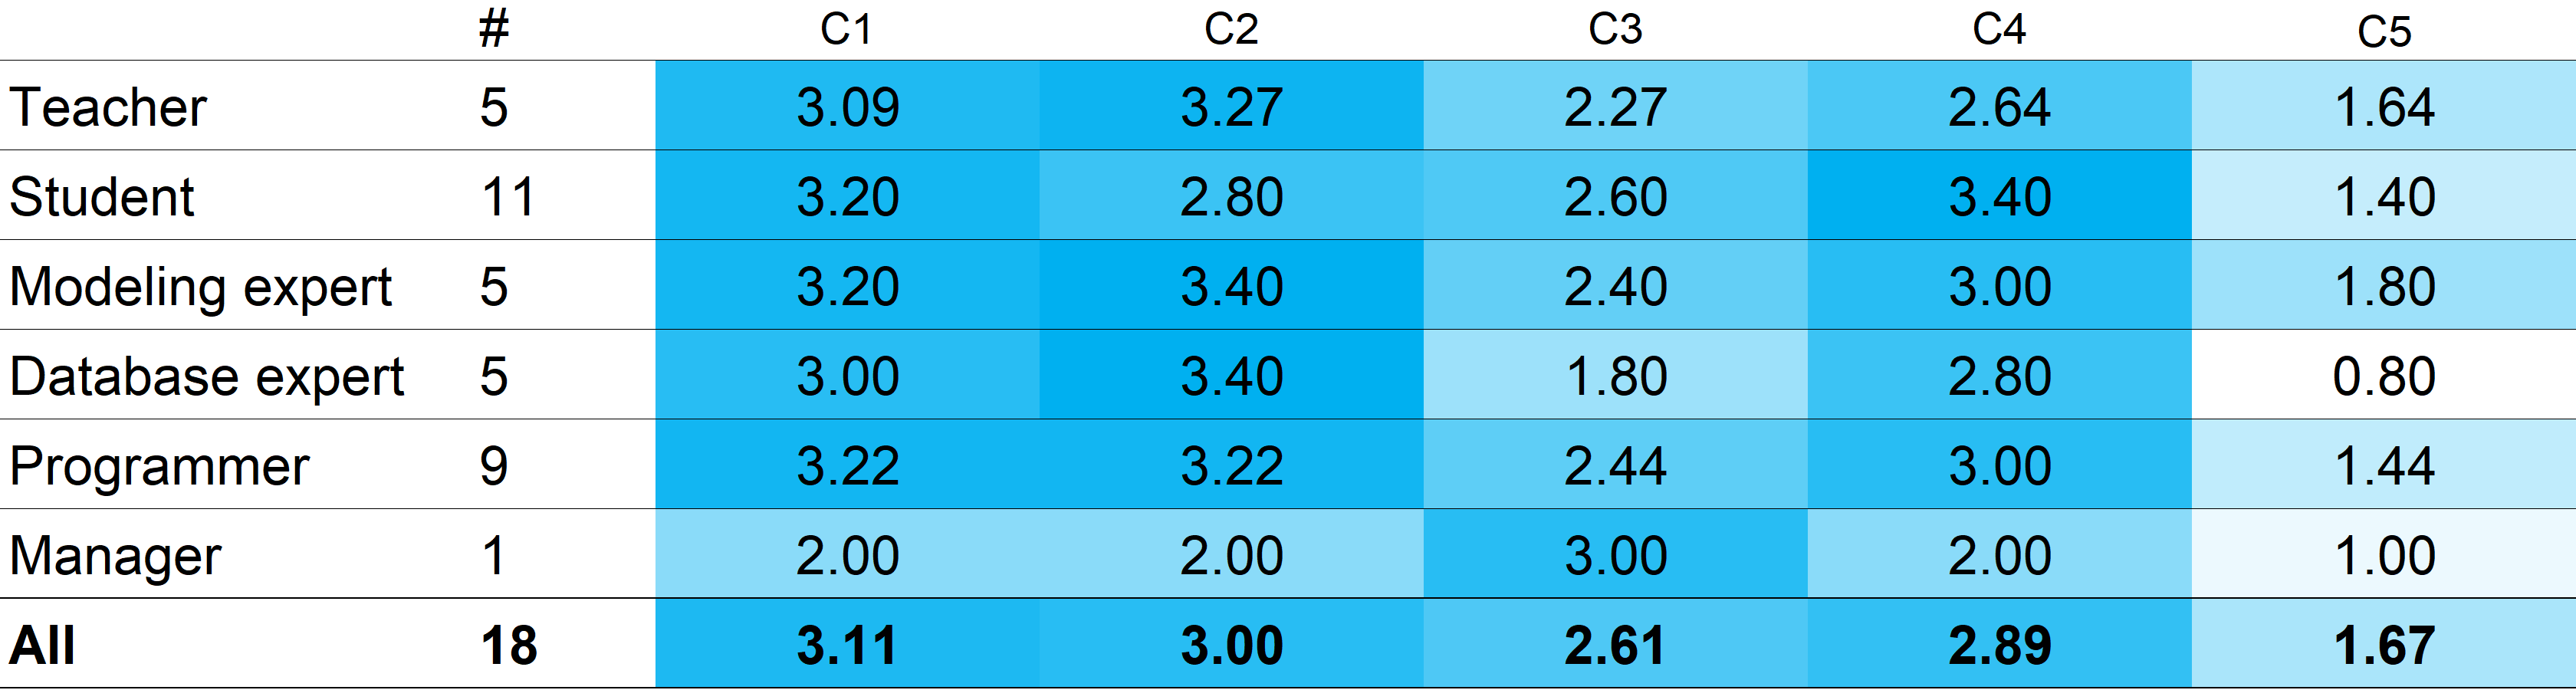
\includegraphics[width=1\linewidth]{img/user-based-evaluation.png} \\
    \scriptsize
\raggedright{C1: Modeling with the assistant is better compared to manual modeling. \\
C2: The assistant is intuitive to use.\\
C3: The assistant suggests appropriate classes, attributes, and associations.\\
C4: The assistant helped me solve the tasks faster compared to manual modeling.\\
C5: I solved all the tasks using only the assistant, and manual modeling was not needed.}
    \caption{Summary of the user-based evaluation. 0=fully disagree, 4=fully agree.}
    \label{fig:user-based-evaluation}
\end{figure}

As we can see, the users agree that using the automated assistant is better than pure manual modeling (C1) and found it intuitive (C2).
The suggestions provided by the tool are subjectively not always appropriate (Q3), which is also supported by our measurements presented in the previous part, and manual modeling is still necessary (Q5).
Despite these imperfections, users claimed that the prototype made them more productive (Q4).
We can find the weakest support in the manager category, but we were able to get only one response in this category, so a further evaluation is necessary.
\chapter{Future work}

\begin{itemize}
\item dynamic domain description
\item adding attribute as an association (and vice versa) and letting LLM suggest a new appropriate name for this attribute/association (NOTE: to možná aspoň trochu udělám)
\item translator of user's plain text instructions into changes inside a conceptual model (TODO: To možná souvisí s tím dynamickým popisem domény, tedy že budeme umět reagovat na změny)
\item in domain description option to highlight the part that the assistant should solely focus on
\item conceptual model updating: assistant that based on some instruction and given conceptual model creates an updated conceptual model (more info: consultation 23)
\item suggestions generation based on chosen ontology design patterns (more info: consultation 23)
\item dání do promptů buď celého uživatelova konceptuálního modelu, nebo pouze nějakých relevantních částí primárně s tím cílem, aby LLM nenavrhoval sémanticky ekvivalentní návrhy a sekundárně ten LLM třeba může použít ten uživatelův konceptuální model k tomu, aby okoukal styl, kterým uživatel modeluje
\end{itemize}


\chapter{Development documentation}
\chapter{Installation documentation}
\chapter{User documentation}
\chapter{Conclusion}
\chapter*{Conclusion}
\addcontentsline{toc}{chapter}{Conclusion}


%%% Bibliography
%%% Bibliography (literature used as a source)
%%%
%%% We employ biblatex to construct the bibliography. It processes
%%% citations in the text (e.g., the \cite{...} macro) and looks up
%%% relevant entries in the bibliography.bib file.
%%%
%%% See also biblatex settings in thesis.tex.

%%% Generate the bibliography. Beware that if you cited no works,
%%% the empty list will be omitted completely.

% We let bibliography items stick out of the right margin a little
\def\bibfont{\hfuzz=2pt}

\printbibliography[heading=bibintoc]

%%% If case you prefer to write the bibliography manually (without biblatex),
%%% you can use the following. Please follow the ISO 690 standard and
%%% citation conventions of your field of research.

% \begin{thebibliography}{99}
%
% \bibitem{lamport94}
%   {\sc Lamport,} Leslie.
%   \emph{\LaTeX: A Document Preparation System}.
%   2nd edition.
%   Massachusetts: Addison Wesley, 1994.
%   ISBN 0-201-52983-1.
%
% \end{thebibliography}


%%% Figures used in the thesis (consider if this is needed)
\listoffigures

%%% Tables used in the thesis (consider if this is needed)
%%% In mathematical theses, it could be better to move the list of tables to the beginning of the thesis.
\listoftables

%%% Abbreviations used in the thesis, if any, including their explanation
%%% In mathematical theses, it could be better to move the list of abbreviations to the beginning of the thesis.
%\chapwithtoc{List of Abbreviations}

%%% Doctoral theses must contain a list of author's publications
\ifx\ThesisType\TypePhD
\chapwithtoc{List of Publications}
\fi

%%% Attachments to the thesis, if any. Each attachment must be referred to
%%% at least once from the text of the thesis. Attachments are numbered.
%%%
%%% The printed version should preferably contain attachments, which can be
%%% read (additional tables and charts, supplementary text, examples of
%%% program output, etc.). The electronic version is more suited for attachments
%%% which will likely be used in an electronic form rather than read (program
%%% source code, data files, interactive charts, etc.). Electronic attachments
%%% should be uploaded to SIS. Allowed file formats are specified in provision
%%% of the rector no. 72/2017. Exceptions can be approved by faculty's coordinator.
\appendix
%\chapter{Attachments}

%\section{First Attachment}

\end{document}
